\documentclass[12pt]{article}
\usepackage{graphicx}
\usepackage{ragged2e}
\usepackage{array}
\usepackage{amsmath,xparse}
\newcolumntype{L}[1]{>{\raggedright\let\newline\\\arraybackslash\hspace{0pt}}m{#1}}
\newcolumntype{C}[1]{>{\centering\let\newline\\\arraybackslash\hspace{0pt}}m{#1}}
\newcolumntype{R}[1]{>{\raggedleft\let\newline\\\arraybackslash\hspace{0pt}}m{#1}}
\begin{document}
	\centering{\bf{KOLHAPUR INSTITUTE OF TECHNOLOGY'S}}\par
	{\bf{COLLEGE OF ENGINEERING (AUTONOMOUS),KOLHAPUR}}
	\par\noindent\rule{\textwidth}{0.4pt}
	
	\centering{\bf{First Year BTech}}\par
	\centering{\bf{MID SEMESTER EXAMINATION}}\par
	\centering{\bf{Engineering Mathematics 1 (123)}}\par
	\begin{flushleft}
		Day and Date :{}\hspace{5.5cm}PRN:
	\end{flushleft}
	
	\begin{flushleft}
		Time :{}\hspace{7cm}Max Marks:{30}\\
	\end{flushleft}
	\noindent\rule{\textwidth}{0.1pt}
\begin{flushleft}
	{\bf Instructions:}\\
	{\hspace{0.5cm} \bf IMP: Verify that you have received question paper with correct course, code, branch, etc}\\
	\hspace{1cm}i) All Questions are Compulsory\\
	\hspace{1cm}ii)Figure to right indicate full marks\\
	\hspace{1cm}iii)Assume suitable data wherever necessary\\
\end{flushleft}

	\begin{flushleft}
	\bf{QNo}\hspace{1.2cm} \bf{Question} \hspace{5.5cm}  \bf{Marks} \hspace{0.2cm} \bf{CO} \hspace{0.2cm}	\bf{BL}	
	
\end{flushleft} 
	\begin{longtable}{|L{1cm}|L{8cm}|C{1cm}|C{1cm}|C{1cm}|}\hline
		\bf{1}. & \bf{Attempt} \bf2 \bf{out} of \bf5 & \bf10  & & \\ \hline
				1.A & The Square of Hypotenus is the sum of squares of 2 adjacent sides. This law is termed as. \newline
					
		A)Euler's law\newline
		B)Pythogaros  Theorem\newline
		C)Newton's Law\newline
		D)Aryabhatta's Law &
		3 &
		CO1&
		1 \\ \hline
		
				1.B & $\frac{1-\cos a}{\sin a}$  equals tp: \newline
					
		A)$\frac{\sin a}{1-\cos a}$\newline
		B)$\frac{\sin a}{1+\cos a}$\newline
		C)$\frac{\cos a}{1-\cos a}$\newline
		D)$\frac{\cos a}{1+\cos a}$ &
		3 &
		CO1&
		2 \\ \hline
		
				1.C & What is the Volume of Cylinder which has radius=4cm and height and 6 cm .$\pi$ =3.14. \newline
					
		A)25\newline
		B)32\newline
		C)25\newline
		D)30 &
		3 &
		CO5&
		4 \\ \hline
		
				1.D & find out the area of triangle with base =3cm and height =4cm. \newline
					
		A)6\newline
		B)12\newline
		C)5\newline
		D)4 &
		3 &
		CO1&
		2 \\ \hline
		
				1.E & find the value of   $y=x^{2}$  where x=4 \newline
					
		A)1\newline
		B)4\newline
		C)9\newline
		D)16 &
		3 &
		CO2&
		3 \\ \hline
		
		
	\end{longtable}

	\begin{longtable}{|L{1cm}|L{8cm}|C{1cm}|C{1cm}|C{1cm}|}\hline
	\bf2. & \bf{Attempt} \bf{2} \bf{out of} \bf{5} & \bf{10}  & & \\ \hline





		2.A &
	Evaluate the following $\int y^{3} dy$ \newline
			
	 &  3 & CO2 & 3\\ \hline
		2.B &
	Rank of the matrix  $\begin{matrix} 1 && 1 &&1 \\ 1 && 1 && 1\\ 1 && 1 && 1 \end{matrix}$ \newline
			
	 &  3 & CO1 & 1\\ \hline
		2.C &
	Differentiate $x^{3}dx$ \newline
			
	 &  3 & CO3 & 1\\ \hline
		2.D &
	Evaluate the following $\int_{2}^{5}\sqrt{\frac{5x}{2}}$ dx \newline
			
	 &  3 & CO3 & 3\\ \hline
		2.E &
	Evaluate $\int \sqrt{5+3x}$ dx \newline
			
	 &  3 & CO3 & 1\\ \hline
	\end{longtable}


\begin{longtable}{|L{1cm}|L{8cm}|C{1cm}|C{1cm}|C{1cm}|}\hline
	\bf3. & \bf{Attempt} \bf{2} \bf{out of} \bf{5} & \bf{10}  & & \\ \hline





		3.A &
	find the sum $\frac{53}{22}+\frac{11}{22}$ \newline
			
	 &  3 & CO1 & 1\\ \hline
		3.B &
	Derive $\pi$ as a ratio of circumfrence and diameter. \newline
			
	 &  3 & CO2 & 4\\ \hline
		3.C &
	Derive the following equation $y=x^{4}$ \newline
			
	 &   & CO2 & 1\\ \hline
		3.D &
	Add the following matrices $\begin{bmatrix} 1 && 2 && 3\\ 4 && 5 && 6\\ 7 && 6 && 4 \end{bmatrix}+\begin{bmatrix} 4 && 5 && 6\\ 7 && 8 && 9 \\ 5 && 4 && 4 \end{bmatrix}$ \newline
			
	 &   & CO1 & 3\\ \hline
		3.E &
	Difference between area of 2 circles \newline
			\begin{center}
		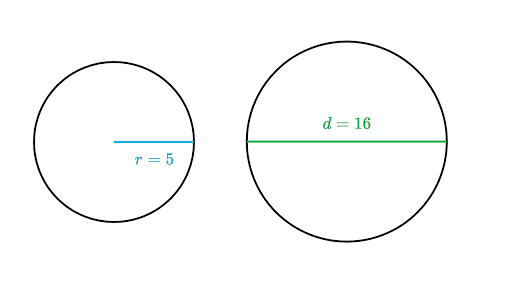
\includegraphics[width=4cm,height=3cm]{media/diagrams/diagram.png}\\\bf{Figure }\bf3.E		
	\end{center}
		
	 &   & CO5 & 1\\ \hline
	\end{longtable}



\end{document}
	
	